% vim:spelllang=en_us:spell

\chapter{Introduction}

When developing software, one commonly relies on software libraries written by
other developers. To avoid introducing defects into the software, one has to
follow rules laid by the library developer. This includes the syntax of the
library and semantics of operations provided by the library. In a concurrent
environment, a new set of problems related to the proper synchronization of
threads is introduced.

\emph{Contracts for concurrency} enable library developers to define
restrictions on the usage of the library in a concurrent environment. In its
basic form, it specifies which method sequences must be executed atomically.
There are two extensions for contracts for concurrency. \emph{Parametric
contracts} allow one to better identify methods that need to be executed
atomically.  Contracts with \emph{spoilers} allow finer control over which
thread interleavings breach the contract. To verify that a program satisfies the
restrictions given by contracts for concurrency, one may use either static or
dynamic analysis, both offering different advantages.

The goal of this project is to design a dynamic analyzer that will be able to
detect contract violations in Java programs. To observe the behavior of the
program under analysis, the program must be modified to report all actions of
interest to the analyzer. That is usually done at the byte code level, and it
requires a lot of skill not to affect the behavior of the program under
analysis. Fortunately, the RoadRunner framework takes care of the instrumenting
and provides a simple interface for observing actions taken by the program under
analysis. The contract analyzer will be built upon the RoadRunner interface.

To successfully perform the analysis, the following must be done. A grammar for
contract definitions and a parser must be created. The instrumentation performed
by RoadRunner needs to be extended to extract additional information about the
program under analysis. Then finally, an analyzer for parametric contracts with
spoilers must be implemented using the RoadRunner interface. This term project
deals with the design of the analyzer and it will be followed by a master's
thesis that will focus on implementation and evaluation of the analyzer.

This report is structured as follows. Chapter \ref{chTwo} describes specifics of
multi-threaded programming in Java, Java memory model, and an overview of
software errors related to concurrency. Approaches to the dynamic analysis of
Java programs and instrumentation techniques are described. Two important
frameworks are presented, the ASM framework for byte code instrumentation, and
the RoadRunner framework for writing dynamic analyzers. Chapter \ref{chThree}
introduces contracts for concurrency, their modified versions, and a method for
dynamic detection of contract violations. In Chapter \ref{chFour}, a dynamic
analyzer for contracts is designed.



\chapter{Dynamic Analysis of Multi-threaded Programs in Java}
\label{chTwo}

This chapter starts with the necessary basics of multithreaded programming in
Java.  The Java Memory Model is introduced, as it defines important terms such
as the \emph{happens-before} relation or a \emph{data race}. Common defects in
a concurrent environment are then described. Section
\ref{approachesToSwVerification} provides an overview of approaches to software
verification.

Dynamic analysis of Java programs is then described, starting with an overview
of Java bytecode, and how it can be instrumented using the ASM framework. The
RoadRunner framework for dynamic analysis is then introduced.


\section{Multi-threaded Programming in Java}

Java provides built-in support for multi-threaded programming. This section
describes a typical thread life cycle, synchronization of threads, and
inter-thread communication, as these are important in dynamic analysis using
contracts.

A thread in Java is represented by a \texttt{Thread} object. There are two ways
to create a thread: by extending the \texttt{Thread} class, or by implementing
the \texttt{Runnable} interface. Both approaches produce a \texttt{Thread}
instance that executes the \texttt{run} method in a new thread when started.

To start a thread, the \texttt{start()} method must be called (which will in
turn call the \texttt{run()} method). The thread will terminate upon returning
from the \texttt{run()} method. The \texttt{join()} method is used in other
threads to wait for a thread to terminate \cite{javaTheCompleteReference}.
Figure \ref{threadExtend} shows a thread creation example by extending the
\texttt{Thread} class, Figure \ref{threadRunnable} shows the same example
achieved by implementing the \texttt{Runnable} interface.

\begin{figure}[hbt]
    \label{threadExtend}
\begin{lstlisting}[language=java]
class MyThread extends Thread {
  @Override
  public void run() {
    System.out.println("This is executed in a new thread.");
  }

  public static void main(String args[]) {
    MyThread t = new MyThread();
    t.start();
    t.join();
  }
}
\end{lstlisting}
    \caption{Creating a thread by extending the \texttt{Thread} class.}
\end{figure}

\begin{figure}[hbt]
    \label{threadRunnable}
\begin{lstlisting}[language=java]
class MyRunnable implements Runnable {
  public void run() {
    System.out.println("This is executed in a new thread.");
  }

  public static void main(String args[]) {
    Thread t = new Thread(new MyRunnable());
    t.start();
    t.join();
  }
}
\end{lstlisting}
    \caption{Creating a thread by implementing the \texttt{Runnable} interface.}
\end{figure}

When accessing a shared resource from multiple threads, proper synchronization
is usually required. In Java, every object gets an implicit monitor, which can
be owned by only one thread at a given time. To enter the monitor, one must use
either synchronized methods or synchronized statements. Synchronized statements
are code blocks with an explicitly specified object whose monitor is entered
before executing the block. Synchronized methods enter the monitor of the
instance they are called upon. Figure \ref{synchronized} shows examples of
synchronized blocks and synchronized methods.

\begin{figure}[hbt]
    \label{synchronized}
\begin{lstlisting}[language=java]
class Example {
  private int a = 0;

  public synchronized void inc1() {
    a++;
  }

  public void inc2() {
    synchronized (this) {
      a++;
    }
  }
}
\end{lstlisting}
    \caption{The \texttt{inc1} method is \emph{synchronized}, on each call, the
    \texttt{Example} instance's monitor is entered. The \texttt{inc2} method is
    not synchronized but contains a \emph{synchronized block} with an explicitly
    specified monitor.}
\end{figure}

Communication between threads is achieved using the following methods:
\texttt{wait()}, \texttt{notify()}, and \texttt{notifyAll()}. All methods must
be called within a synchronized context. Calling \texttt{wait()} will suspend
the calling thread until some other thread enters the same monitor and calls
either \texttt{notify()} or \texttt{notifyAll()}.

Multi-threaded programs may use the \texttt{volatile} type modifier. It tells
the compiler that the variable may be modified outside of the current thread.
\todo{elaborate}

\section{Java Memory Model}

% http://www.cs.umd.edu/~pugh/java/memoryModel/jsr-133-faq.html
% https://docs.oracle.com/javase/specs/jls/se8/html/jls-17.html#jls-17.4.5

\emph{Java memory model} describes how threads in Java interact with each other
using shared memory. The model takes a program and an execution trace, and for
each read operation decides if it is valid or not. The decision depends on the
write operation that modified the data before the read operation. The compiler,
runtime, and hardware must ensure that all executions of a program produce
execution traces that are valid according to the model \cite{jmmspec}.

In a single-threaded program, it is only required that the program produces the
same result as if it was run serially. The compiler is free to reorder
instructions when it does not affect the result of the computation.

In multi-threaded programs, the reordering of instructions has to be limited
when the threads interact with each other. In the model, only certain program
\emph{actions} are considered. There are several orders defined over the actions
which are used by the dynamic contract analysis: \emph{program order},
\emph{synchronization order}, and \emph{happens-before order}.

The actions can be either \emph{intra-} or \emph{inter-thread}. An inter-thread
action can be detected or influenced by another thread. An intra-thread action
is for example adding two local variables and it is not important to the model.
Non-volatile reading or writing of a shared variable is an inter-thread action.
\emph{Synchronization actions} are inter-thread actions that include volatile
reading or writing of variables, locking and unlocking of monitors, and starting
and stopping of a thread. Figure \ref{threadActions} shows examples of different
kinds of actions.

\begin{figure}[hbt]
    \label{threadActions}
\begin{lstlisting}[language=java]
class MySharedData {
  int mySharedVar = 0;

  public synchronized void MyMethod() {
    // synchronization action (entering a monitor)
    // intra-thread action (writing a local variable)
    int a = 42;
    // 2 inter-thread actions (reading and writing a shared variable)
    mySharedVar += a;
    // synchronization action (leaving a monitor)
  }
}
\end{lstlisting}
    \caption{Different program actions classified from the Java Memory Model
    point of view. Entering and leaving \texttt{MyMethod} produces
    \emph{synchronization actions}. Accessing \texttt{mySharedVar} is considered
    as an \emph{inter-thread} action, but not as a synchronization action
    because \texttt{mySharedVar} is not declared as \texttt{volatile}.}
\end{figure}


\emph{Program order} is a total order over all inter-thread actions from a given
thread. It reflects the order in which these actions would be executed if
run by the intra-thread semantics.

\emph{Synchronization order} is a total order over all synchronization actions
of an execution. Within each thread, the synchronization order is consistent
with the program order. The \emph{synchronized-with} relation is defined on
certain actions. For example: starting a thread is \emph{synchronized-with}
the first action in the new thread.

\emph{Happens-before order} is a partial order. If an action
\emph{happens-before} another, the first action is visible to and ordered before
the second action. If actions \emph{x} and \emph{y} belong to the same thread
and \emph{x} comes before \emph{y} in program order, then \emph{x happens-before
y}.  If \emph{x synchronizes-with y}, then \emph{x happens-before y}. Figures
\ref{hb1} and \ref{hb2} illustrates the \emph{happens-before} relation in simple
programs.

A \emph{data race} occurs, when there are two accesses to the same variable, at
least one of which is write, and these accesses are not ordered by
\emph{happens-before}. This situation is illustrated in Figure \ref{hb2}.

\begin{figure}[hbt]
    \label{hb1}
    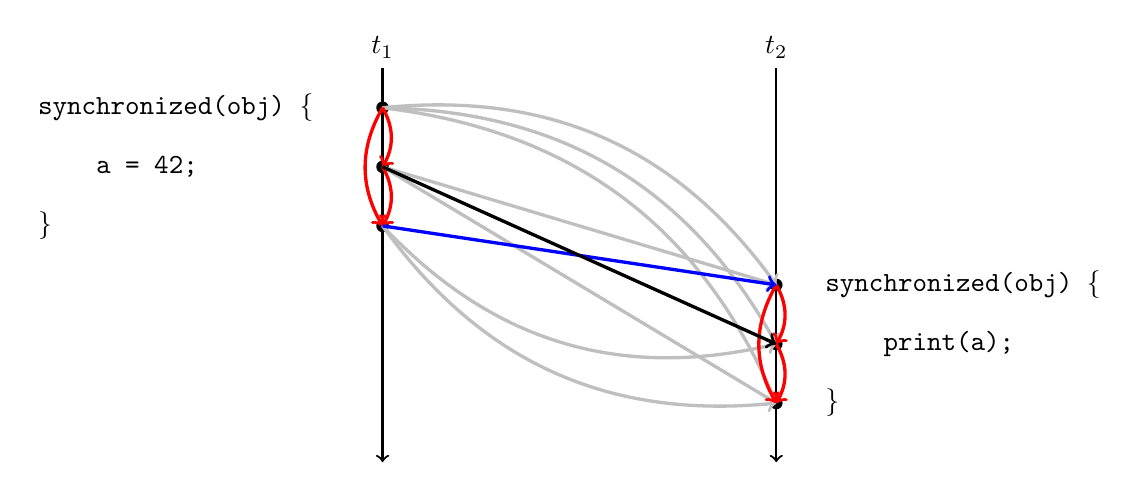
\begin{tikzpicture}
    \draw [->, thick] (4.5,0.5) node[above] {$t_1$} -- (4.5,-4.5);
    \draw (0,0) node[right] {\texttt{synchronized(obj) \{}};
    \coordinate (a1) at (4.5,0);
    \fill (a1) circle (0.08);
    \draw (0,-0.75) node[right] {\texttt{\quad \quad a = 42;}};
    \coordinate (a2) at (4.5,-0.75);
    \fill (a2) circle (0.08);
    \draw (0,-1.5) node[right] {\texttt{\}}};
    \coordinate (a3) at (4.5,-1.5);
    \fill (a3) circle (0.08);

    \draw [->, thick] (9.5,0.5) node[above] {$t_2$} -- (9.5,-4.5);
    \draw (10,-2.25) node[right] {\texttt{synchronized(obj) \{}};
    \coordinate (b1) at (9.5,-2.25);
    \fill (b1) circle (0.08);
    \draw (10,-3) node[right] {\texttt{\quad \quad print(a);}};
    \coordinate (b2) at (9.5,-3);
    \fill (b2) circle (0.08);
    \draw (10,-3.75) node[right] {\texttt{\}}};
    \coordinate (b3) at (9.5,-3.75);
    \fill (b3) circle (0.08);

    \draw[->,color=lightgray,very thick] (a1) to[bend left] (b1);
    \draw[->,color=lightgray,very thick] (a1) to[bend left] (b2);
    \draw[->,color=lightgray,very thick] (a1) to[bend left] (b3);
    \draw[->,color=lightgray,very thick] (a2) to (b1);
    \draw[->,color=lightgray,very thick] (a2) to (b3);
    \draw[->,color=lightgray,very thick] (a3) to[bend right] (b2);
    \draw[->,color=lightgray,very thick] (a3) to[bend right] (b3);

    \draw[->,color=red,very thick] (a1) to[bend left] (a2);
    \draw[->,color=red,very thick] (a2) to[bend left] (a3);
    \draw[->,color=red,very thick] (a1) to[bend right] (a3);

    \draw[->,color=red,very thick] (b1) to[bend left] (b2);
    \draw[->,color=red,very thick] (b2) to[bend left] (b3);
    \draw[->,color=red,very thick] (b1) to[bend right] (b3);

    \draw[->,color=blue,very thick] (a3) to (b1);

    \draw[->,very thick] (a2) to (b2);
\end{tikzpicture}

    \caption{\emph{Happens-before} relations in a correctly synchronized program
    consisting of threads $t_1$ and $t_2$. Each arrow represents a
    \emph{happens-before} relation. The red arrows represent the program order,
    the blue arrow represents the \emph{synchronizes-with} relation. Grey arrows
    complete the transitive closure. The conflicting accesses to variable
    \texttt{a} are not a data race, because they are ordered by
    \emph{happens-before} (the black arrow).}
\end{figure}

\begin{figure}[hbt]
    \label{hb2}
    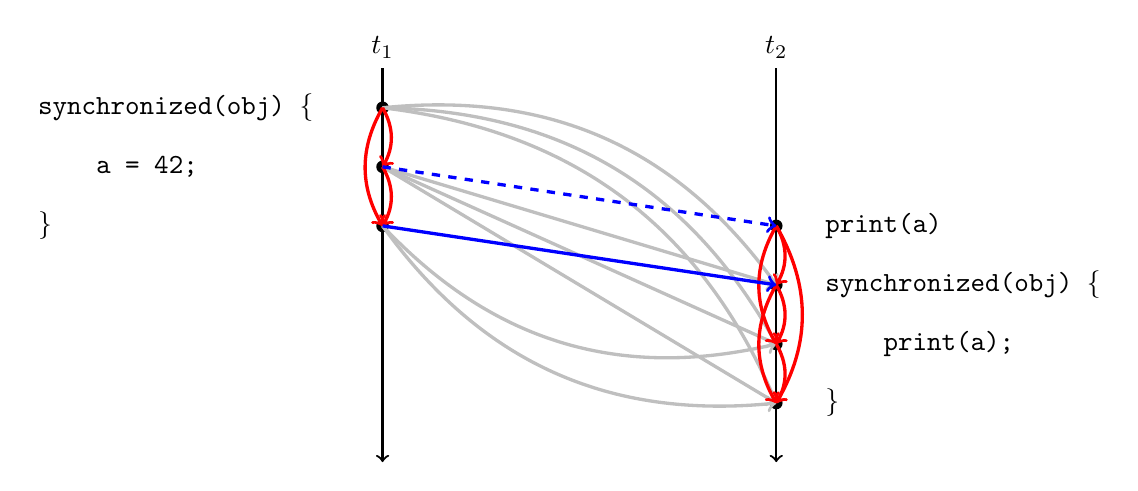
\begin{tikzpicture}
    \draw [->, thick] (4.5,0.5) node[above] {$t_1$} -- (4.5,-4.5);
    \draw (0,0) node[right] {\texttt{synchronized(obj) \{}};
    \coordinate (a1) at (4.5,0);
    \fill (a1) circle (0.08);
    \draw (0,-0.75) node[right] {\texttt{\quad \quad a = 42;}};
    \coordinate (a2) at (4.5,-0.75);
    \fill (a2) circle (0.08);
    \draw (0,-1.5) node[right] {\texttt{\}}};
    \coordinate (a3) at (4.5,-1.5);
    \fill (a3) circle (0.08);

    \draw [->, thick] (9.5,0.5) node[above] {$t_2$} -- (9.5,-4.5);
    \draw (10,-1.5) node[right] {\texttt{print(a)}};
    \coordinate (b0) at (9.5,-1.5);
    \fill (b0) circle (0.08);
    \draw (10,-2.25) node[right] {\texttt{synchronized(obj) \{}};
    \coordinate (b1) at (9.5,-2.25);
    \fill (b1) circle (0.08);
    \draw (10,-3) node[right] {\texttt{\quad \quad print(a);}};
    \coordinate (b2) at (9.5,-3);
    \fill (b2) circle (0.08);
    \draw (10,-3.75) node[right] {\texttt{\}}};
    \coordinate (b3) at (9.5,-3.75);
    \fill (b3) circle (0.08);

    \draw[->,color=lightgray,very thick] (a1) to[bend left] (b1);
    \draw[->,color=lightgray,very thick] (a1) to[bend left] (b2);
    \draw[->,color=lightgray,very thick] (a1) to[bend left] (b3);
    \draw[->,color=lightgray,very thick] (a2) to (b1);
    \draw[->,color=lightgray,very thick] (a2) to (b2);
    \draw[->,color=lightgray,very thick] (a2) to (b3);
    \draw[->,color=lightgray,very thick] (a3) to[bend right] (b2);
    \draw[->,color=lightgray,very thick] (a3) to[bend right] (b3);

    \draw[->,color=red,very thick] (a1) to[bend left] (a2);
    \draw[->,color=red,very thick] (a2) to[bend left] (a3);
    \draw[->,color=red,very thick] (a1) to[bend right] (a3);

    \draw[->,color=red,very thick] (b0) to[bend left] (b1);
    \draw[->,color=red,very thick] (b0) to[bend right] (b2);
    \draw[->,color=red,very thick] (b0) to[bend left] (b3);
    \draw[->,color=red,very thick] (b1) to[bend left] (b2);
    \draw[->,color=red,very thick] (b2) to[bend left] (b3);
    \draw[->,color=red,very thick] (b1) to[bend right] (b3);

    \draw[->,color=blue,dashed,very thick] (a2) to (b0);

    \draw[->,color=blue,very thick] (a3) to (b1);
\end{tikzpicture}

    \caption{\emph{Happens-before} relations in an incorrectly synchronized
    program (each solid arrow represents a \emph{happens-before} relation).
    There is no \emph{happens-before} relation between conflicting accesses
    \texttt{a=42} and \texttt{print(a)} (the dashed line), creating a data race.}
\end{figure}


\section{Safety Errors in Multi-threaded Programs}

When compared to single-threaded programs, multi-threaded programs may encounter
a whole new class of errors related to sharing memory between threads. Errors
presented in this section are classified as \emph{safety errors} in \cite{letko}
as these are usually checked in various dynamic analyses.

\paragraph{Data Race}
A \emph{data race} occurs when there are two unsynchronized accesses to a shared
variable and at least one of them is a write access.

\paragraph{Atomicity Violation}
When a code block is required to be atomic, all
program executions must be equivalent to an execution where the block is
executed serially.

\paragraph{Order Violation}
When certain operations are required to be executed
in a certain order, and the order is not met in a given program execution, an
\emph{order violation} occurs.

\paragraph{Deadlock}
General definition of a deadlock is presented in
\cite{letko}. A program state contains a set $S$ of deadlocked threads if, and
only if each thread in $S$ is blocked and waiting for some event that could
unblock it, but such an event could only be generated by a thread from $S$.

\paragraph{Missed Signal}
A \emph{missed signal} is present in a program execution when one or more
threads are waiting for a signal, and the signal is never delivered.

\section{Approaches to Software Verification}
\label{approachesToSwVerification}

% Carlo Ghezzi, Mehdi Jazayeri, Dino Mandrioli: Fundamentals of Software Engineering, Prentice Hall, ISBN 0-13-099183-X

The goal of software verification is to make sure that the software meets all
requirements. This section provides a summary of testing, dynamic and static
analysis, abstract interpretation, theorem proving, and model checking.

\paragraph{Testing}
\emph{Testing} consists of running the software under different conditions and
checking the results of the computation (or observing other behavior of the
software). To gain enough confidence that the software operates correctly in all
conditions, a suitable set of \emph{test cases} must be found, which is
difficult, and sometimes impossible. Testing is best suited for confirming
the presence of defects in software, not for proving their absence
\cite{fundamentals}.

An important property of test cases is their \emph{repeatability}, meaning that
a certain test case will always yield the same result. When testing
multi-threaded programs, this property does not hold because of the
non-determinism introduced by the thread scheduler. Threads are interleaved
differently on each execution which means that errors may or may not appear.
This makes discovering defects in multi-threaded programs difficult.

\paragraph{Dynamic Analysis}
\emph{Dynamic analysis} works with information gathered during an execution of a
program. The information may be analyzed during program execution
(\emph{on-the-fly}) or at the end (\emph{post-mortem}). Even though the analysis
works with information from a single execution, it can in some cases find errors
that were not observed during the execution but may demonstrate themselves in
similar executions \cite{letko}. The dynamic analysis also suffers from
nondeterministic scheduling. The program under analysis may also behave
differently due to being observed by the analyzer.

\paragraph{Static Analysis}
\emph{Static analysis} is performed at compile-time and it does not require the
program to be running. The analysis is theoretically able to cover all possible
executions of a program. In practice, it is limited by the fact that the number
of thread interleavings in multi-threaded programs grows exponentially
\cite{letko}.

\paragraph{Abstract Interpretation}
\emph{Abstract interpretation} takes the source code and symbolically executes
it line by line, approximating the semantics of the program without performing
all the calculations. It suffers from similar problems as static analysis.

\paragraph{Model Checking}
\emph{Model checking} is a technique for checking whether a system satisfies
certain correctness specification \cite{letko}. It is based on systematic or
heuristic exploration of the state space. The drawback of this technique is that
the state space of the program model can be huge.

\paragraph{Theorem Proving}
\emph{Theorem proving} is a semi-automated approach to proving that a certain
facts are satisfied in the system. It is based on assumptions and general
theorems about the system and uses mathematical reasoning.

\section{Instrumentation of Java Bytecode}

Instrumentation is the act of inserting instructions into an existing program to
extract useful information at runtime. Instrumentation can be used to measure
performance, log events, or perform dynamic analysis. The running program should
not be aware that it is being instrumented and the result of the computation
should remain the same. Instrumentation may add significant overhead to the
program. For example, programs instrumented by the RoadRunner framework are
roughly 10 times slower \cite{RoadRunner}.

In Java, the instrumentation is done by changing the bytecode. There are several
general-purpose frameworks for modifying the Java bytecode. In this section, the
ASM framework is described as it is used by the RoadRunner framework, which is
the basis of this master's thesis.

\subsection{Java Bytecode Overview}

Programs written in Java are compiled into Java bytecode which is executed by
the Java Virtual Machine. Every class gets compiled into a Java class file
containing the following sections \cite{asmguide}:
\begin{itemize}
    \item Section with information about the class itself, such as the name of
    the class, the super class, implemented interfaces, and class annotations.
    \item One section per field, containing the field name, type, modifiers, and
    annotations.
    \item One section per method (and constructor), containing the name of the
    method, the return type, type of parameters, annotations, and compiled code
    of the method.
\end{itemize}

Java class files also contain a \emph{constant pool} section that holds all
numeric, type, and string constants which are then referenced from other
sections of the file. The whole structure is shown in Table \ref{classfile}.
The Java class file format is described in detail in the Java Virtual Machine
Specification \cite{jvmspec}.

\begin{table}
    \begin{center}
        \label{classfile}
        \begin{tabular}{|l|l|l|}
            \hline
            \multicolumn{2}{|l|}{Modifiers, name, super class, interfaces} \\
            \hline
            \multicolumn{2}{|l|}{Constant pool} \\
            \hline
            \multicolumn{2}{|l|}{Annotations} \\
            \hline
            \multicolumn{2}{|l|}{Attributes} \\
            \hline
            \multirow{3}{*}{Fields} & Modifiers, name, type \\
            & Annotations \\
            & Attributes \\
            \hline
            \multirow{3}{*}{Methods} & Modifiers, name, return and parameter types \\
            & Annotations \\
            & Attributes \\
            & Code \\
            \hline
        \end{tabular}
        \caption{Structure of the Java class file. Adapted from \cite{asmguide},
        simplified.}
    \end{center}
\end{table}

The Java Virtual Machine operates on two kinds of types: \emph{primitive types}
and \emph{reference types}. Examples of primitive types are \texttt{int},
\texttt{long}, \texttt{boolean}, or \texttt{double}. There are three kinds of
reference types: class types, array types, and interface types. The array type
consists of a component type which can also be an array type. For example,
\texttt{int[]} represents an array type with component type of \texttt{int}. All
reference types may hold a special null reference, which is also the default
value of reference types.

Compiled classes do not contain any \texttt{package} or \texttt{import}
statements, so all type names must be fully qualified. Internally, class files
use slashes instead of dots in type names, so for example
\texttt{java.lang.Object} becomes \texttt{java/lang/Object}. In most places,
Java types are represented with \emph{type descriptors}. Each primitive type is
assigned a single character: \texttt{I} for \texttt{int}, \texttt{D} for
\texttt{Double}, and so on. Classes and interfaces are written with prefix
\texttt{L} and semicolon at the end, so \texttt{String} becomes
\texttt{Ljava/lang/String;}. Arrays are represented using a
\texttt{\leftbracket} and the element type, so an array of integers is
\texttt{\leftbracket I}, an array of strings is \texttt{\leftbracket
Ljava/lang/String;}. Similarly, \emph{method descriptors} are used to represent
the return type of a method and types of all method parameters. For example, a
method declared as \texttt{double m(int i, String s)} would be represented as
\texttt{(ILjava/lang/String;)D}. In method descriptors, \texttt{V} is used when
the method returns \texttt{void}.

When executing, on each method invocation, the Java Virtual Machine creates a
new \emph{frame}. Each frame contains its own local variables and an operand
stack. When the method invocation is completed, the frame is destroyed.

Local variables are addressed by indexing. Each variable can hold a single value
of a primitive or reference type with the exception of \texttt{long} and
\texttt{double} which require a pair of variables. At index 0, there is a
reference to the object the method was invoked on (the value of \texttt{this} in
Java). Class methods (marked as \texttt{static} in Java) do not use this index.
Starting at index 1 (or 0 in case of class methods), method parameters are
stored. After the parameters, local variables may be stored.

Each frame contains an \emph{operand stack}, which is initially empty. Various
instructions are used to load values onto the stack, either from local variables
or fields. Other instructions take operands from the stack and push the result
back. When calling other methods, the parameters are also prepared on the stack.

Java Virtual Machine instructions can be divided into several categories. Load
and store instructions move values between local variables and the operand
stack. For example, instruction \texttt{iload\_3} pushes the value (which is of
type \texttt{int}) from the local variable at index 3 to the operand stack.
Arithmetic instructions usually take two values from the operand stack, compute
the result, and store it back on the stack. For example, instruction
\texttt{fmul} will multiply two values of type \texttt{float}. Type conversion
instructions convert the value on the top of the stack. Control transfer
instructions, such as \texttt{ifeq} or \texttt{goto}, cause the execution of
instruction other then the immediately following.

To create new arrays and objects, instructions \texttt{new}, \texttt{newarray},
and \texttt{anewarray} are used. Methods are invoked using these five
instructions: \texttt{invokevirtual}, \texttt{invokeinterface},
\texttt{invokespecial}, \texttt{invokestatic}, and \texttt{invokedynamic}, each
used in slightly different circumstances. Exceptions are thrown using the
\texttt{athrow} instruction. An example of a method represented by bytecode is
shown in Figure \ref{bytecodeExample}.

\begin{figure}[hbt]
    \label{bytecodeExample}
    \begin{lstlisting}
public void foo(java.io.FileWriter, int, int)
  descriptor: (Ljava/io/FileWriter;II)V
  flags: (0x0001) ACC_PUBLIC
  Code:
    stack=2, locals=5, args_size=4
       0: iload_2
       1: iload_3
       2: iadd
       3: istore        4
       5: aload_1
       6: iload         4
       8: invokevirtual #2    // Method java/io/FileWriter.write:(I)V
      11: aload_1
      12: invokevirtual #3    // Method java/io/FileWriter.close:()V
      15: return
    \end{lstlisting}
    \caption{An example of a method bytecode viewed using the \texttt{javap}
    command. The method takes three parameters: a file writer and two integers.
    There are 5 local variables: the object the method was called on (index 0),
    method parameters (indices 1 to 3), and a local variable (index 5). On lines
    0 to 3, the two integers are loaded on to the operand stack, added together,
    and the result is stored in a local variable. Lines 5 to 7 calls the
    \texttt{write} method on the file writer, lines 11 and 12 calls the
    \texttt{close} method. Operands on lines 8 and 12 are indices to the
    constant pool section.}
\end{figure}


\subsection{The ASM framework}

The ASM framework allows generating and modifying Java classes directly in
bytecode. It can be used both statically (for example during compilation) or
dynamically (to create classes at runtime). The ASM framework provides an
interface for loading and storing the bytecode using higher-level abstractions,
such as constants, identifiers, methods, fields, etc. \cite{asmguide}.

There are two interfaces available: the \emph{core API} with an
\emph{event-based} representation of classes, and the \emph{tree API} with an
\emph{object-based} representation. The core API processes classes sequentially.
When parsing a class, the ASM parser will produce an event for each element of
the class.  When writing a class, the writer creates the class based on a
sequence of events. The tree API loads the whole class and creates a tree of
objects representing the class. The core API is faster and requires less memory,
however, it is not practical for complex transformations \cite{asmguide}. The
RoadRunner framework uses the core API.

The core API is based on the \texttt{ClassVisitor} abstract class. The class
contains methods for visiting different sections of a class, for example,
\texttt{visitAttribute}, \texttt{visitMethod}, or \texttt{visitField}. Complex
sections, such as methods or fields, have their visitor classes. For example,
the \texttt{MethodVisitor} class contains methods such as
\texttt{visitLocalVariable}, \texttt{visitCode}, or \texttt{visitParameter}
\cite{asmguide}.

To generate a new class, one has to create a \texttt{ClassWriter} instance,
which is a subclass of \texttt{ClassVisitor}. Then a sequence of visit methods
must be called, such as \texttt{visitField} or \texttt{visitMethod}. The
\texttt{ClassWriter} instance will generate appropriate bytecode on each call.

To read and parse a class, one has to create a \texttt{ClassReader} instance.
The reader will produce a sequence of events for each section of the class. To
consume those events, a \texttt{ClassVisitor} instance must be given to the
reader. The reader will then call appropriate visit methods on the visitor as it
is parsing the class. To demonstrate this, one can create a \texttt{ClassReader}
and connect it to a \texttt{ClassWriter} (which is a subclass of
\texttt{ClassVisitor}). The reader will call visit methods on the writer,
effectively copying the class.

\begin{figure}[hbt]
    \label{asmArchitecture}
    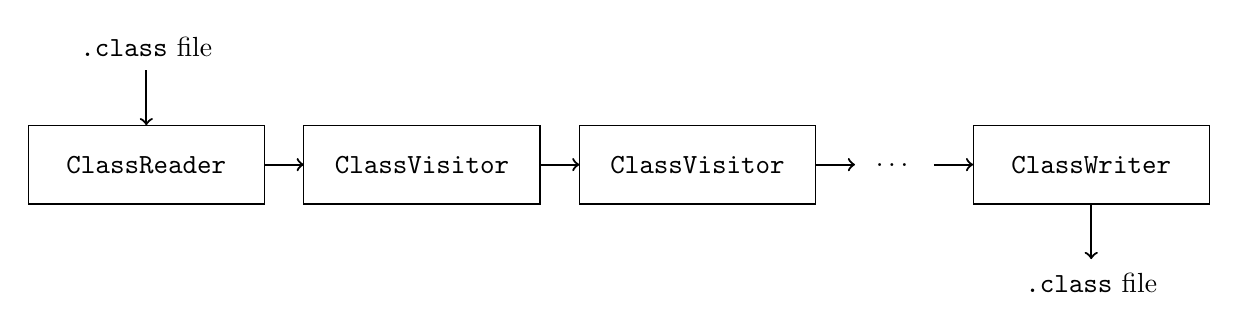
\begin{tikzpicture}
    \draw (0,1.5) node {\texttt{.class} file};
    \draw [->, thick] (0,1.2) -- (0,0.5);
    \draw (-1.5,0.5) rectangle (1.5,-0.5);
    \draw (0,0) node {\texttt{ClassReader}};
    \draw [->, thick] (1.5,0) -- (2,0);
    \draw (2,0.5) rectangle (5,-0.5);
    \draw (3.5,0) node {\texttt{ClassVisitor}};
    \draw [->, thick] (5,0) -- (5.5,0);
    \draw (5.5,0.5) rectangle (8.5,-0.5);
    \draw (7,0) node {\texttt{ClassVisitor}};
    \draw [->, thick] (8.5,0) -- (9,0);
    \draw (9.5,0) node {\ldots};
    \draw [->, thick] (10,0) -- (10.5,0);
    \draw (10.5,0.5) rectangle (13.5,-0.5);
    \draw (12,0) node {\texttt{ClassWriter}};
    \draw [->, thick] (12,-0.5) -- (12,-1.2);
    \draw (12,-1.5) node {\texttt{.class} file};
\end{tikzpicture}

    \caption{Typical architecture for class transformation.}
\end{figure}

The typical class transformation uses the following architecture (see Figure
\ref{asmArchitecture}): a \texttt{ClassReader} instance reads the class, then
one or more \texttt{ClassVisitor} instances modify the class, and then a
\texttt{ClassWriter} instance writes the modified class back to a file.

\section{Dynamic Analysis using RoadRunner}

The RoadRunner framework is used for the dynamic analysis of concurrent programs
written in Java. RoadRunner instruments programs to obtain a stream of events
that are useful for dynamic analysis, such as memory accesses, synchronizing on
a lock, forking or joining of threads, and so on. This event stream is then
available to various analysis tools. Multiple tools can be chained together,
each tool acting as a filter over the events. This allows complex analyses to be
built from simpler, modular tools \cite{RoadRunner}.

RoadRunner aims to simplify writing dynamic analysis tools. A RoadRunner
analysis tool only needs to handle events of interest. RoadRunner will ensure
that the event is properly detected and the event handler is called. To store
the state of the analysis, RoadRunner provides support for associating data with
memory locations, locks, or threads.

\todo{tool composition}
\todo{optional: debugging, comparing analyses}

\subsection{The RoadRunner Programming Interface}

Every analyzer in RoadRunner is based on the \texttt{Tool} class. Figure
\ref{toolclass} contains the most important methods of \texttt{Tool}. During the
analysis, every time an action is detected, the appropriate method in
\texttt{Tool} is called, along with an \texttt{Event} object that contains
information about the event.

\begin{figure}[hbt]
    \label{toolclass}
    \begin{lstlisting}[language=java]
public abstract class Tool {
  // event handlers for accessing a memory location
  public void access(AccessEvent fae) { }
  public void volatileAccess(VolatileAccessEvent fae) { }
  // event handlers for entering and exiting methods
  public void enter(MethodEvent me) { }
  public void exit(MethodEvent me) { }
  // event handlers for locking
  public void acquire(AcquireEvent ae) { }
  public void release(ReleaseEvent re) { }
  // event handlers for thread events
  public void preJoin(JoinEvent je) { }
  public void postJoin(JoinEvent je) { }
  public void preStart(StartEvent se) { }
  public void postStart(StartEvent se) { }
  // shadow location initialization
  public ShadowVar makeShadowVar(AccessEvent ae) { }
}
    \end{lstlisting}
    \caption{The abstract class \texttt{Tool}. Only selected public methods are
    shown.}
\end{figure}

The following events are detected by the RoadRunner framework:
\begin{itemize}
    \item Method entry and exit.
    \item Memory accesses -- reads and writes to fields and variables.
    \item Lock acquires and releases.
    \item Synchronization signals -- wait and notify.
    \item Thread forking and joining.
\end{itemize}

There are several subclasses of the \texttt{Event} class with specific
information about events.

RoadRunner allows associating data with objects from the program under analysis.
For each thread, a \texttt{ShadowThread} object is created which contains a
reference to the underlying thread. Similarly, for each lock, a
\texttt{ShadowLock} object is created. Both extend the \texttt{Decoratable}
class that allows storing of arbitrary information. For associating data with
memory locations, a \emph{shadow location} is created when the location is first
accessed.

Multiple tools can be chained together. Each event handler method forwards the
\texttt{Event} instance to the next tool in the chain by default. If the event
is not forwarded, the tool becomes a filter over the event stream. This can be
used to filter out events that are not interesting to a particular analysis and
then performing the analysis in the next tool.

\subsection{Instrumentation Performed by RoadRunner}

RoadRunner uses a modified version of the ASM framework to instrument the
program under analysis.

\todo{how are fields instrumented}

\todo{how are methods instrumented}


\chapter{Contracts for Concurrency}
\label{chThree}

When developing software, one frequently uses modules created by someone else
via its programming interface. For example, in object-oriented programming, the
interface consists of public methods of a given class. Accessing the interface
requires one to follow a protocol consisting of: (i) syntax, i.e. types of
parameters and return values, (ii) semantics, i.e. the expected behavior for
given input parameters, and (iii) access restrictions. Access restrictions
include the domain of valid values, dependencies on other services, and
atomicity violations \cite{contracts}.

\emph{Contracts for concurrency} \cite{FITPUB10817},
\cite{DBLP:journals/corr/SousaDFL15}, are a case of a software protocol that
expresses access restrictions in a concurrent setting. In its basic form, it
specifies sequences of methods that must be executed atomically. The contracts
can be extended with parameters to reflect the data flow between the methods (so
that only methods manipulating the same data must be executed atomically).
Another extension adds so-called \emph{spoilers} (so that given sequence must be
executed atomically only with respect to only certain sequences). Both
extensions can be combined \cite{contracts}. This chapter defines basic
contracts, as well as both extensions to them. Then a method for dynamic
validation of contracts for concurrency is presented.

\section{Basic Contracts}
\label{basicContracts}

A \emph{contract} is formally defined in \cite{FITPUB10817} as follows. Let
$\Sigma_\mathbb{M}$ be a set of all public method names (the API) of a module or
a library. A \emph{contract} is a set $\mathbb{R}$ of \emph{clauses}. Each
clause $\varrho \in \mathbb{R}$ is a star-free regular expression over
$\Sigma_\mathbb{M}$. A contract violation occurs when any of the sequences in a
contract is interleaved with an execution of a method from $\Sigma_\mathbb{M}$
over the same object.

\emph{Example.} Consider a map implementation with the following operations:
\texttt{put(key, value)}, \texttt{get(key)}, \texttt{remove(key)}, and
\texttt{contains(key)}. Then a contract for this class may contain the following
clauses:
\begin{align*}
    (\varrho_1) &\ \texttt{put get}\\
    (\varrho_2) &\ \texttt{contains (put|get|remove)}
\end{align*}
Clause $\varrho_1$ states that when an element is put into the map and then
retrieved, it should be executed atomically (because the element may be removed
between the calls). Clause $\varrho_2$ states that when the program modifies the
map based on the result of the \texttt{contains} call, it should be atomic.

\section{Parametric Contracts}
\label{parametricContracts}

In some situations, the definition of contracts may be too restrictive,
producing false alarms. In \cite{contracts}, contracts are extended with
parameters to reflect the data flow between methods. Consider the following
example:
\begin{lstlisting}[language=java]
if (q.contains(42)) q.remove(42);
\end{lstlisting}

These two calls must be executed atomically only if they share the same
argument. This dependency can be expressed using \emph{meta-variables} placed as
the parameters or return values of methods. Parameters that should not be taken
into account are marked with free meta-variable (denoted with an underscore).

\emph{Example.} The example from section \ref{basicContracts} can be extended
with parameters:
\begin{align*}
    (\varrho_1) &\ \texttt{put(X) \_ = get(X)}\\
    (\varrho_2) &\ \texttt{\_ = contains(X) ( put(X,\_) | \_ = get(X) |
    remove(X) )}
\end{align*}

The basic definition of contracts contains one implicit parameter, the object
that the method was called upon (\texttt{this} in Java) \cite{FITPUB10817}. To
better illustrate this, the example can be rewritten as:
\begin{align*}
    (\varrho_1) &\ \texttt{X.put(Y) \_ = X.get(Y)}\\
    (\varrho_2) &\ \texttt{\_ = X.contains(Y) ( X.put(Y,\_) | \_ = X.get(Y) |
    X.remove(Y) )}
\end{align*}


\section{Contracts with Spoilers}
\label{contractsWithSpoilers}

In \cite{contracts}, contracts are extended with contextual information to
distinguish which method sequences violate the contract. Each clause of the
basic contract is called a \emph{target} and is assigned a set of so-called
\emph{spoilers}. A spoiler is a set of method sequences that may violate its
target.

Consider clause $\varrho_1$ from the example in section \ref{basicContracts}. If
the element that was put into the map is concurrently removed or updated before
the \texttt{get} call, a contract violation should be detected.  However,
calling \texttt{contains} or \texttt{get} on the element will not affect the
computation and should not be marked as a contract violation. In this example,
methods \texttt{put} and \texttt{remove} are spoilers for a target
$\varrho_1$, denoted as \texttt{put get} $\leftsquigarrow$ \texttt{put|remove}.

% TODO: this is basically copied - is it ok?

Formally, as defined in \cite{contracts}, let $\mathbb{R}$ be the set of
\emph{target} clauses where each target $\varrho \in \mathbb{R}$ is a regular
expression over $\Sigma_\mathbb{M}$. Let $\mathbb{S}$ be the set of
\emph{spoilers} where each spoiler $\sigma \in \mathbb{S}$ is a regular
expression over $\Sigma_\mathbb{M}$. A \emph{contract} is a relation $\mathbb{C}
\subseteq \mathbb{R} \times \mathbb{S}$ defining for each target, which spoilers
may cause atomicity violation.

Contract violation is observed when a target sequence $\varrho \in \mathbb{R}$
is fully interleaved by a spoiler sequence $\sigma \in \mathbb{C}(\varrho)$ and
the sequences are executed on the same object.

\emph{Example.} The example from section \ref{basicContracts} can be extended
with spoilers:
\begin{align*}
    (\varrho_1) &\ \texttt{put get} \leftsquigarrow \texttt{put|remove}\\
    (\varrho_2) &\ \texttt{contains (put|get|remove)} \leftsquigarrow
    \texttt{put|remove}
\end{align*}

When combining parametric contracts with spoilers, the spoilers may also contain
parameters. Then a contract violation is detected only when spoiler arguments
match target arguments.

\emph{Example.} Examples from sections \ref{parametricContracts} and
\ref{contractsWithSpoilers} combined together:
\begin{align*}
    (\varrho_1) &\ \texttt{X.put(Y) \_ = X.get(Y)} \leftsquigarrow
    \texttt{X.put(Y,\_)|X.remove(Y)}\\
    (\varrho_2) &\ \texttt{\_ = X.contains(Y) ( X.put(Y,\_) | \_ = X.get(Y) |
    X.remove(Y) )}\\
    &\quad \leftsquigarrow \texttt{X.put(Y,\_)|X.remove(Y)}
\end{align*}


\section{Dynamic Contract Validation}

In \cite{contracts}, a dynamic contract validation method is proposed for
contracts with spoilers. Parametric contracts are not included in the method.
This section provides an overview of the method.

\subsection{Multi-threaded Program Traces}

In context of the dynamic contract validation, multi-threaded program
\emph{trace} consists of events of the following types:
\begin{itemize}
    \item thread forking or joining another thread,
    \item thread entering or exiting a method,
    \item thread acquiring or releasing a lock.
\end{itemize}

All events in a trace are indexed by their position in the trace. Let
$\mathbb{T}$ be a set of threads, $\mathbb{R}$ a set of targets, $\mathbb{S}$ a
set of spoilers, $\mathbb{C} \subseteq \mathbb{R} \times \mathbb{S}$ a set of
contracts, and $\mathbb{L}$ a set of locks. The set of all events that can be
generated by a thread $t \in \mathbb{T}$ is then denoted as $\mathbb{E}_t$. Let
$\mathbb{E} = \bigcup_{t \in \mathbb{T}} \mathbb{E}_t$. A \emph{trace} is then a
sequence $\tau = e_1 \hdots e_n \in \mathbb{E}^+$.

% TODO: basically copied

Given a trace $\tau = e_1 \hdots e_n \in \mathbb{E}^+$, we call its subsequence
$r = e_{i_1} e_{i_2} \hdots e_{i_k}$, $1 < k \leq n$, an \emph{instance} of a
target $\varrho \in \mathbb{R}$ if, and only if:
\begin{enumerate}
    \item $r$ consists of well-paired method enter and exit events,
    \item all enter events of $r$ match the regular expression of $\varrho$,
    \item apart from events $e_{i_1},\ldots,e_{i_k}$, there is no event from the
        alphabet of $\varrho$ executed by $t$ between events $e_{i_1}$ and
        $e_{i_k}$.
\end{enumerate}

\emph{Example.} Given target $\varrho = abc$, and a trace $\tau_1 = adbdc$,
there is a target instance $r = e_1 e_3 e_4$. In trace $\tau_2 = acbdc$, there
is no target instance.

A \emph{spoiler instance} $s$ of a spoiler $\sigma \in \mathbb{S}$ is defined
similarly. We let $start(r) = e_{i_1}$ and $end(r) = e_{i_k}$ denote the first
and last events of a target, respectively. Likewise, $start(s)$ and $end(s)$
denotes the first and last events of a spoiler, respectively.

\subsection{Contract Violation}

A contract is violated when there is a target instance that is fully interleaved
with a spoiler instance. The interleaving is defined using a
\emph{happens-before} relation, which is in the context of contracts defined as
follows \cite{contracts}. A \emph{happens-before relation} $\prec_{hb}$ over a
trace $\tau = e_1 \ldots e_n \in \mathbb{E}^+$ is the smallest transitively
closed relation on the set of events from $\tau$ such that $e_j \prec_{hb} e_k$
holds when $j < k$ and one of the following holds:
\begin{enumerate}
    \item both $e_j$ and $e_k$ are executed by the same thread,
    \item both $e_j$ and $e_k$ acquire or release the same lock,
    \item one of $e_j$ and $e_k$ is a fork or a join performed by thread $t$,
        and the other is executed by thread $u$.
\end{enumerate}

A contract $(\varrho,\sigma) \in \mathbb{C}$ is \emph{violated} in a trace
$\tau$ if, and only if there is a target instance $r$ in the trace and a spoiler
instance $s$ in the trace such that:
\begin{align*}
    start(s) \nprec_{hb} start(r) \wedge end(r) \nprec_{hb} end(s)
\end{align*}
The violation occurs when the spoiler may have started after the target started
and it may have ended before the target ended. When given a complete program
execution trace, all target and spoiler instances can be detected, the
happens-before relation can be deduced, and all contracts can be easily checked
for violations. The trace, however, can get large and make this approach
unpractical. For this reason, several optimizations are introduced in
\cite{contracts}, which are presented in the next section.

% TODO: examples of traces

\subsection{On-the-fly Contract Validation}

To check contract validations, it is not required to keep the entire program
execution trace. A \emph{trace window} is kept instead. Events are moved to the
trace window as soon as they become available and are removed under certain
conditions. The goal is to keep the window as small as possible.

Spoiler instances can be safely removed from the window whenever a contract
violation that would be detected with the spoiler can be detected without it. A
spoiler instance can be removed from the window whenever a newer instance of the
same spoiler is detected \cite{contracts}.

A target instance $r$ can be safely removed with respect to a spoiler instance
$s$ whenever a contract violation that would be detected between $r$ and $s$,
can be detected between $s$ and another target instance too. Note that target
instances may be removed only with respect to a given spoiler, not in general
\cite{contracts}.

To further reduce the required information about the trace, \emph{vector clocks}
are used. For each target and spoiler instance in the trace window, only vector
clocks of their beginning and end need to be kept.

The method for contract validation on-the-fly does the following. At method
entry events, target and spoiler sequences are detected. At method exit events,
it is detected whether a target or a spoiler instance has ended. When a target
instance ends, spoiler instances from the trace window are checked if they
violate the target. When a spoiler instance ends, target instances from the
trace window are checked if they are violated by the spoiler. At method exit,
target and spoiler instances are also discarded when no longer needed.



\chapter{Design of a Dynamic Analyzer for Parametric Contracts with Spoilers}
\label{chFour}

This chapter describes the proposed dynamic analyzer for parametric contracts
with spoilers. The analyzer should follow the method for dynamic analysis of
contracts described in \cite{contracts} and extend it to support parametric
contracts.

\todo{chapter overview}

The analyzer should be built as a new tool (or a toolchain) for RoadRunner. The
input will be a program under analysis and a contract definition. The analyzer
will be able to detect contract violations in the program and report them. The
RoadRunner framework will be modified to support obtaining method arguments and
return values. For performance reasons, the RoadRunner framework should also be
modified to instrument only relevant actions of the program under analysis.

\section{Restricting Parametric Contracts}

The analyzer should work with parametric contracts with spoilers (see Chapter
\ref{chThree}). For performance reasons, the analyzer will validate only a
restricted variant of contracts. It is required that the value of all parameters
in target or spoiler sequences must be determined by the first method in the
sequence. For example, method sequence \texttt{a(X,Y) b(Y,Z)} is illegal,
because after the call to method \texttt{a}, the value of parameter \texttt{Z}
is still unknown. Free meta-variables (\texttt{\_}) do not have to be
determined. For example, the sequence \texttt{a(X,Y) b(\_) c(Y)} is valid. This
restriction will limit the number of instances in the trace window.

The method described in \cite{contracts} is based on program traces where
every method represents a single event in the trace. However, the RoadRunner
framework produces two events for every method -- method entry and method exit.
Method arguments are available on method entry, the return value is available on
method exit. The analyzer must work around the fact that the return value (which
can be also a parameter) is not available at the method entry. Alternatively,
the contracts should be limited to not use parametrized return values.

\todo{overlapping instances}

\section{Contract Representation}

The analyzer takes a contract definition as a parameter. At the top level, the
definition will contain target spoiler pairs. Each target and spoiler will be
represented by a regular expression over methods. Each method will be
parametrized, including arguments, return value, and the object it is called
upon (\texttt{this}).

Method in contracts must be specified unambiguously. Method names must be fully
qualified (for example \texttt{java.lang.Object.toString}). Java allows method
overloading, so the contract definition should allow for distinguishing methods
based on the number and type of their parameters. It should be possible to
include a constructor in a contract.

\todo{grammar for contract configuration files}

Internally, each target and spoiler will be converted from a regular expression
to a finite automaton, represented by the \texttt{FiniteAutomaton} class, where
each transition contains a method definition and parameters.

\section{Changes to Instrumentation Performed by RoadRunner}

The RoadRunner framework does not expose the method arguments or the return
value through its API. The \texttt{enter} and \texttt{exit} methods both take a
\texttt{MethodEvent} parameter containing the following information:
\begin{itemize}
    \item Target -- \texttt{null} for static methods, the value of \texttt{this}
        for instance methods.
    \item A \texttt{MethodInfo} object -- static information about the method
        definition (name, descriptor, whether it is synchronized or static).
    \item Call site location -- where was the method invoked.
\end{itemize}

The \texttt{MethodEvent} class should be extended for storing method arguments
and the return value. In RoadRunner, each method call is wrapped in another, so
RoadRunner has access to these values. RoadRunner does not need to provide
argument types, since they are already available in the method descriptor
(stored in \texttt{MethodInfo}). Also, the analysis performs only identity
comparison (in the case of objects). Primitive types must be handled correctly
and compared by their value.

For dynamic analysis of contracts for concurrency, only a subset of all events
is required. The RoadRunner framework should be configured or modified to
instrument only the necessary actions of the program under analysis. Event types
that are not used at all, such as memory accesses, should not be instrumented.
Method entries and exits should be instrumented only in case the method is part
of a contract.

\section{A Contract Validator Tool}

The contract analyzer should be implemented as a subclass of the \texttt{Tool}
class. The following methods will be overridden:
\begin{itemize}
    \item \texttt{enter()} and \texttt{exit()}, for detecting spoiler and target
        instances;
    \item \texttt{acquire()} and \texttt{release()}, for detecting
        synchronization between threads;
    \item \texttt{create()}, for creating shadow data for the new thread;
    \item \texttt{preStart()}, for initializing shadow data;
    \item \texttt{postJoin()}, for thread synchronization after joining.
\end{itemize}

Methods for detecting memory accesses will not be used by the analyzer, and also
no data will be stored in shadow memory locations.

For each thread, a \texttt{ShadowThread} object will be created that will store
a \emph{vector clock} for the thread, and information about target and spoiler
instances. For each lock, a \texttt{ShadowLock} object will be created that will
store a vector clock for the lock.

The vector clocks associated with threads and locks will be updated on actions,
that impose a happens-before order of operations between threads. Forking or
joining thread will update both threads' vector clocks. When a thread acquires a
lock, the thread's vector clock is updated. When a lock is released, its vector
clock is updated. The sole purpose of \texttt{acquire()}, \texttt{release()},
\texttt{create()}, \texttt{preStart()}, and \texttt{postJoin()} methods is to
update various vector clocks.

Methods \texttt{enter()} and \texttt{exit()} will track target and spoiler
instances in a thread, and detect contract violations.

\subsection{Detection of Target and Spoiler Instances}

For each thread, a \texttt{Window} object is kept during the analysis. It
contains a reference to the thread, a vector clock, and information about target
and spoiler instances present in the trace window. An instance contains a
reference to the spoiler or target finite automaton, the current state of the
automaton, and the values of parameters.

When a window is created, for each target and spoiler, an empty \emph{template}
instance is added that will be used for detecting new instances in the trace
window. These instances will remain unchanged during the lifetime of the window.

On method entry, the analyzer will try to advance all instances in a window.
When a template instance can be advanced, it means that a new instance is
detected. The template instance is copied, the value of parameters is stored in
the instance, and the instance is advanced to the next state. When an already
running instance can be advanced, the analyzer must check if the method
arguments match those stored in the instance.

\subsection{Contract Validation}

On method exit, for all target instances that were just fully accepted, it is
checked if there is a spoiler instance in other windows that can violate this
target. Likewise, for all accepted spoiler instances, it is checked if there is
a target instance in other windows that can be violated by this spoiler. If a
violation is found, it is reported and the analysis ends. If not, the instance
is replaced by a template instance, which contains the same finite automaton,
parameter values, and vector clocks of the instance that has just ended. This
ensures that when a new instance with the same parameter values is detected, it
will have access to the previously detected instance.

\todo{synchronization of the tool itself}

\section{Testability}

To properly test the analyzer, its implementation should not rely on
RoadRunner's internal data structures. It should be possible to feed the
analyzer a custom event stream without the need for the RoadRunner framework.



\chapter{Implementation}
\label{chFive}

\todo{TODO}



\chapter{Conclusion}

The goal of this term project was to design a dynamic analyzer for validating
parametric contracts with spoilers. The first part of this report provides the
necessary background for designing an extension to the RoadRunner framework.
Multi-threading in Java, Java Memory Model, and Java bytecode is described.
Then the contracts for concurrency, along with their extensions, were presented.
Finally, a dynamic analyzer for parametric contracts with spoilers was designed.
It will be implemented as an extension to the RoadRunner framework.  Necessary
changes to the RoadRunner itself were described.

A master's thesis that will follow the term project will focus on implementing
the analyzer and on testing it on real-world programs.
